\chapter{Introduction}
\section{Problem Statement}
%\indent{
\hspace*{0.82cm}Today smart phones are not exclusive property of early adopters or IT professionals.
Global Smart phone shipments grew a relatively healthy 43 per cent year-over-year to reach
600 million units in Q2 2010. According to comScore’s report, 234 million Americans
subscribed to mobile phone plans in January 2010. Of these 42.7 million owned internet
accessible smart phones, this represented an 18 per cent increase over the three months ended
in October.\\[0.5cm]
\hspace*{0.82cm}Important progress in mobile computing should start with straightforward local
convergence of Smartphones and computer infrastructure via simplistic mobile use model.
This use model would enhance the current synchronization schemes by by-passing the
synchronized data over proprietary services and giving the user the full control and full
accessibility of his/her own data both on the smart phone, as well on his very own
synchronization server. It is not always advisable for users to use synchronization services
provided by Google for android devices.\\[0.5cm]
\hspace*{0.82cm}These services may not ensure full privacy of all the data of the user. This data is
stored on the Google clouds. Also, today the security issues in cloud computing have not
been fully resolved. Hence it cannot be said our data remains fully secure when it is on
Google premises. Synchronization can be done by various means by the use of this product.
Offline and online mode synchronization is possible. Online mode can be used when user is
on-the-go and offline synchronization may be used when user is at the office or at home.\\[0.5cm]
%}
\section{Project Objective}
\hspace*{0.82cm}The project addresses the idea of android smartphones being synchronized in an
online and offline manner. A server application in the form of a desktop application and a
client application in the form of an android application is to be developed to achieve this
objective.\\[0.5cm]
The basic objectives of the project include:
\begin{itemize}
%\begin{spacing}{0}{
 \item Setting up a secure online connection of the mobile phone to the server.
 \item Setting up interfacing techniques to connect the mobile phones to the PC via a USB
cable, Bluetooth link or Wi-Fi.
 \item Devising a protocol which will control the authentication of the device, flow of data
in and out of the smartphone and the server.
 \item Managing user account on the server application.
 \item Developing the application such that it is cross-platform compatible i.e. it can be
deployed on a PC running any OS – Linux, Mac OSX or Windows.
%}\end{spacing}
\end{itemize}

\section{Architecture of the System}
\subsection{Current system}
\hspace*{0.82cm}The current system being used for synchronization involves the data being
synchronized to be synced via a Google account the user has to maintain. This means data
will have to be given to a third-party provider like Google when it actually not really
necessary to do so.\\[0.5cm]
This scenario is illustrated in figure 1.1.

\begin{figure}[H]
  \centering
    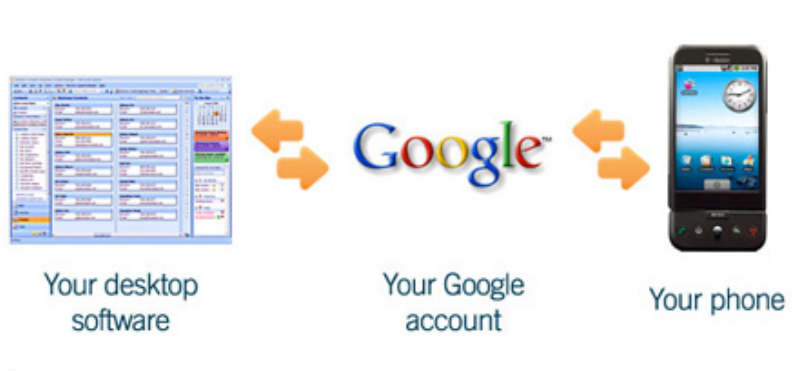
\includegraphics[height= 5cm, width=13cm]{project/images/architecture-current}
  \caption{\textbf{Architecture of Current System}}
\end{figure}

It is not always possible to store sensitive information on third-party premises 
like Google. This sensitive information can be in the form of phone logs, SMS, 
contacts, e-mails, notes, calendar schedules, etc.

\subsection{Proposed System}
\hspace*{0.82cm}The proposed system enables Android mobile device to be synchronized by the user
using this product such that all data may be synchronized in a private mutually exclusive
manner. This is illustrated in figure 1.2.

\begin{figure}[H]
  \centering
    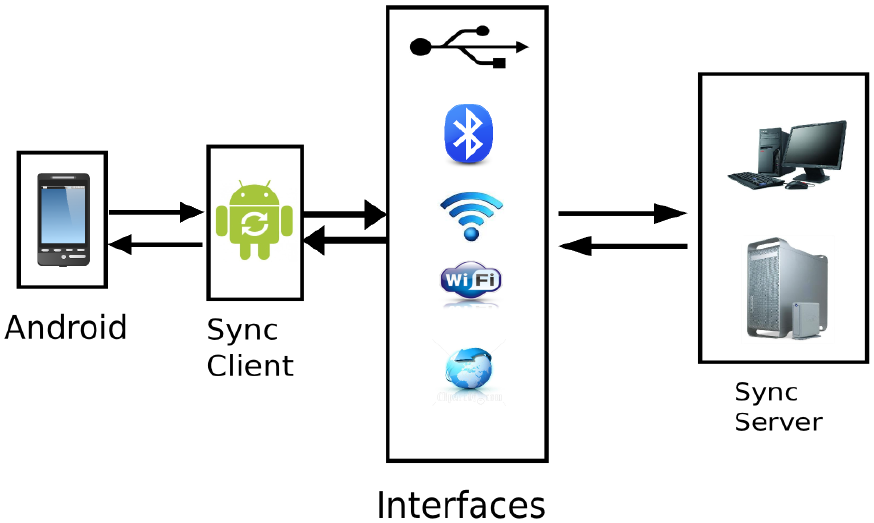
\includegraphics[height= 7cm, width=15cm]{project/images/architecture-proposed}
  \caption{\textbf{Architecture of Proposed System}}
\end{figure}

In this system, the android smartphone is connected to the server and after the
connections is established, synchronization may be started using any mode- offline or online
i.e. using a Cable or Wi-Fi or over a secure internet connection.